\documentclass[conference]{IEEEtran}

\usepackage[brazilian]{babel}
\usepackage[utf8]{inputenc}
\usepackage[T1]{fontenc}
\usepackage{enumerate}


\ifCLASSINFOpdf
   \usepackage[pdftex]{graphicx}
   \graphicspath{{../pdf/}{../jpeg/}}
   \DeclareGraphicsExtensions{.pdf,.jpeg,.png}
\else
   \DeclareGraphicsExtensions{.eps}
\fi



\begin{document}

\title{Autenticação de Usuários através de uma abordagem Abordagem Orientada a Serviços e o protocolo LDAP v3}%

% author names and affiliations
% use a multiple column layout for up to three different
% affiliations
\author{
\IEEEauthorblockN{Everton de Vargas Agilar}
\IEEEauthorblockA{Computer Centre of UnB\\
University of Brasília\\
Brasília, Brazil\\
evertonagilar@unb.br}

\and

\author{
\IEEEauthorblockN{Renato Carauta}
\IEEEauthorblockA{Computer Centre of UnB\\
University of Brasília\\
Brasília, Brazil\\
renatocarauta@unb.br}

}


\maketitle

% As a general rule, do not put math, special symbols or citations
% in the abstract
\begin{abstract}
A modernização dos sistemas legados é um processo que vem ganhando 
cada vez mais interesse na Universidade de Brasília (UnB). 
Entre os desafios envolvidos na condução da modernização na UnB, 
pelo seu Centro de Informática (CPD), destaca-se a ausência de 
integração entre as aplicações e as duplicidades de componentes que implementam lógica de negócio. Assim, 
é imprescindível que, enquanto a modernização seja realizada, os novos sistemas sejam integrados aos antigos, de forma a 
interagir e compartilhar os seus fluxos de negócios. A Arquitetura Orientada a Serviços (SOA) surge como uma maneira de solucionar 
este problema, disponibilizando uma abstração de alto nível entre as aplicações e a camada de negócio.
Este artigo descreve os resultados preliminares de uma 
dissertação de mestrado que objetiva propor e validar uma 
abordagem orientada a serviços que compreende um processo 
de moderniza\c c\~{a}o e um barramento aderente ao estilo 
arquitetural \textit{Representational State Transfer} (REST). 
Esta abordagem visa sustentar a integração dos fluxos de informações e minimizar 
as duplicidades de lógica de negócios existentes entre as aplicações, através de um barramento  orientado a serviço, 
para que possa auxiliar o CPD na modernização dos sistemas legados da Instituição, que estão em uso há mais de 20 anos.
\end{abstract}

\section{Introdução}

A modernização dos sistemas 
legados tem lugar quando as 
tradicionais práticas de manutenção deixam de 
atender \`{a}s organizações. Entre os objetivos que se buscam com a modernização, 
podem-se citar a redução dos custos com manutenção, maior integração entre os sistemas e torná-los mais flexíveis às mudanças, 
de forma a prolongar sua vida útil~\cite{S4_bennett1995legacy,S3_Bisbal:1999,S15_Comella-DordaASurvey2000}. 

Do ponto de vista das organizações, os sistemas legados correspondem às aplicações que sustentam o funcionamento 
negocial de uma instituição e que consolidam a maior parte das informações corporativas~\cite{S3_Bisbal:1999}. 
Nesse contexto, a modernização dos sistemas legados ganha cada vez mais importância 
para a Universidade de Brasília (UnB), uma vez que, 
nos últimos 20 anos, uma gama considerável de sistemas foi desenvolvida. 
São sistemas com um arcabouço de regras de negócio que foram sendo 
construídas ao longo dos anos e que são de vital importância para o pleno funcionamento da Universidade. 
Entretanto, durante o ciclo de vida desses sistemas, 
ocorreram várias revisões para mantê-los alinhados com as necessidades da Instituição, 
tornando-os mais rígidos e inflexíveis, 
a ponto de serem de difícil manutenção. 

Os sistemas da Universidade dividem-se em três áreas de negócio: área de gestão acadêmica, administrativa e de pessoal. 
A maioria desses sistemas estão sob diferentes linguagens de programação, arquiteturas e plataformas; e não conversam entre
si, a não ser, por meio do banco de dados. Durante muitos anos, a linguagem de programação predominante foi o Visual Basic. 
Dois dos sistemas mais importantes estão escritos nessa linguagem: Sistema de
Informações e Gestão Acadêmica (SIGRA) e o Sistema de
Informações de Pessoal (SIPES). Os demais sistemas foram
desenvolvidos em VB.NET, C\#, PHP, ASP e Java (plataforma atual). 

Este artigo apresenta os resultados iniciais de uma disserta\c c\~{a}o 
de mestrado que tem como objetivo propor uma abordagem para apoiar 
a modernização dos sistemas legados da Universidade, 
com vistas a diminuir a duplicidade de implementa\c c\~{a}o 
de regras de negócio entre as aplicações (um dos problemas mais 
críticos relacionados à qualidade do software desenvolvido pelo 
CPD). Essa abordagem deve atender a alguns requisitos, tais como: (a) 
seguir uma estrat\'{e}gia orientada a serviço e  
aderente a arquitetura \textit{Representational State Transfer} (REST); 
(b) apresentar uma curva de aprendizagem aceitável, para que possa ser 
realmente implantada no CPD; e oferecer bons mecanismos de disponibilidade, 
escalabilidade e monitoramento.

Mais especificamente, aqui são descritos os principais resultados alcançados 
até esse momento:

\begin{itemize}
\item a caracterização do termo modernização de software, alcançado com a 
condução de um mapeamento sistemático (Seção~\ref{ms}). 

\item a implementação de um protótipo arquitetural de um barramento 
orientado a serviços (Seção~\ref{arquitetura}), cujas decisões de projeto atende aos 
requisitos de alta disponibilidade, escalabilidade e monitoramento.  
\end{itemize} 

Este artigo também apresenta o planejamento de um 
estudo empírico (Seção~\ref{estudo-empirico}) que está sendo 
conduzido com o envolvimento dos alunos matriculados em uma disciplina da pós-graduação 
relacionada a análise estática e engenharia reversa de software. 




\section{Modernização de Software}\label{ms}

A condução de mapeamento sistemático (MS) na área de 
Engenharia de Software tem se tornado uma prática 
consolidada que envolve um conjunto bem definido 
de atividades~\cite{Petersen:2008}. Esta seção descreve 
o resultado da primeira análise realizada no MS com o intuito de caracterizar a modernização dos sistemas legados no contexto da manutenção de software, ao identificar 
as principais contribuições e estudos na literatura sobre este tema. Mais detalhes deste estudo foram submetidos ao \textit{The 31st ACM/SIGAPP Symposium on Applied Computing} (ACM SAC 2016). Para tal estudo, um protocolo de estudo foi elaborado, de modo a permitir sua reprodução por outros pesquisadores, sem os problemas do viés de publicação mencionados em~\cite{kitchenham:2004}.

\subsection{An\'{a}lise Relacionada à Primeira Questão de Pesquisa}

A modernização pode ser caracterizada, de acordo com~\cite{S01_bennett2000software, S9_bianchi:2003, S3_Bisbal:1999, S15_Comella-DordaASurvey2000, S2_erlikh:2000}, pela necessidade de evolução dos sistemas para adequá-lo aos requisitos de negócio das organizações, seja com novas funcionalidades, correção de erros ou atualizações tecnológicas. Nesse sentido, muitas teorias tem sido sugeridas na literatura, como discutido a seguir. 

\textbf{N. Weiderman et al.} introduzem um modelo de ciclo de vida 
para descrever a evolução de um sistema durante a sua vida útil~\cite{S15_Comella-DordaASurvey2000, Seacord:2003, S12_WeidermanApproaches:1997}. 
Neste modelo, existem três fases distintas: manutenção, modernização e substituição.  Nesse ciclo, as necessidades de negócio da organização são intercaladas com as implementações realizadas para suprir essas necessidades. 
Além de introduzir um modelo de ciclo de vida, Weiderman et al. também propõem distinguir a modernização pelo nível de compreensão requerido para suportar 
os esforços de modernização: \textit{White-box} para compreensão das estruturas internas do sistemas e \textit{Black-box} quando requer a compreensão das interfaces externas dos sistemas legados.

\textbf{K. Bennett et al.} propõem um modelo chamado 
\textit{staged model} para descrever o ciclo de vida de um sistema e auxiliar na identificação das principais 
áreas de pesquisa sobre modernização~\cite{S01_bennett2000software}. Este modelo divide-se em 5 etapas: 
\textit{initial development, evolution, servicing, phase-out, close-down}. Aqui, a modernização compreende a fase \textit{evolution} e, 
ao contrário do modelo proposto por Weiderman et al., é considerada uma atividade de manutenção, que pode ser classificada em 
4 classes: adaptativa, quando há alterações no ambiente do software; perfectiva, para novos requerimentos do usuário; corretiva, correção de erros; e preventiva, para 
prevenir problemas futuros. 

\textbf{J. Bisbal et al.} apresentam um modelo de ciclo de vida, onde o foco são as atividades evolutivas ordenadas pelo impacto causado nos 
sistemas~\cite{S3_Bisbal:1999}. Assim, dividem-se em \textit{wrapping}, cujo objetivo é prover uma nova interface para os componentes de um sistema, 
tornando-os mais acessíveis para outros componentes; manutenção, para os pequenos ajustes e correção de erros; a migração, que visa mover o sistema 
legado para um ambiente mais flexível, mantendo os dados e funcionalidades originais; e o redesenvolvimento, que reescreve por completo as aplicações. 

Percebe-se que, embora esses modelos usem termos distintos para referir-se as fases do ciclo de vida dos sistemas, há várias semelhanças. Por exemplo, 
o significado de substituição ~\cite{S15_Comella-DordaASurvey2000, Seacord:2003, S12_WeidermanApproaches:1997} é o mesmo que redesenvolvimento ~\cite{S3_Bisbal:1999} e o significado de migração ~\cite{S3_Bisbal:1999} é o mesmo que modernização ~\cite{S15_Comella-DordaASurvey2000, Seacord:2003, S12_WeidermanApproaches:1997}. No entanto, 
a fase \textit{wrapping} descrita por Bisbal et al. é uma técnica de modernização \textit{Black-box} em Weiderman et al. ~\cite{S15_Comella-DordaASurvey2000, Seacord:2003, S12_WeidermanApproaches:1997}.

Com a caracterização da modernização de software, finaliza-se esta análise com um \textit{word cloud}, disponível na figura ~\ref{fig:word_cloud}, dos 30 termos mais citados nos \textit{abstracts} das fontes primárias selecionadas para o MS. Note que, sob a perspectiva tecnol\'{o}gica, \'{e} poss\'{i}vel perceber nessa figura um certo grau de interesse na computa\c c\~{a}o orientada a servi\c cos. 


\begin{figure}
\centering
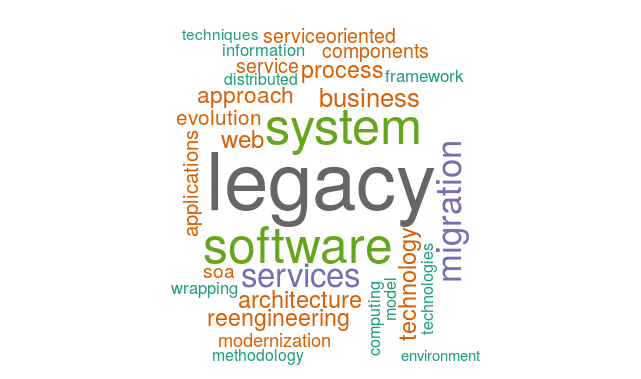
\includegraphics[scale=0.5]{figuras/word_cloud.png}
\caption{Termos mais citados nas publicações selecionadas}
\label{fig:word_cloud}
\end{figure}

\section{Arquitetura}\label{arquitetura}

Esta seção apresenta a arquitetura do barramento (intitulado ErlangMS) que está 
sendo proposto para apoiar as atividades de modernização 
de software do CPD. 

O ErlangMS é um barramento orientado a serviço (\textit{Enterprise Service Bus}, ESB) 
que est\'{a} sendo desenvolvido na linguagem Erlang. O barramento 
fornece a camada de serviço para a abordagem SOA proposta neste trabalho. De acordo 
com \cite{SOAPractice:2007}, um ESB possibilita o uso de serviços, unificando o acesso a esses serviços através de uma camada intermediadora entre componentes de software (denominados serviços) e as aplicações 
que consomem estes serviços.

Nesse sentido, ErlangMS foi idealizado para servir de elo entre os 
sistemas da Universidade e a camada de negócio (tipicamente 
implementada usando a linguagem Java). A implementa\c c\~{a}o 
de um novo barramento (em vez da ado\c c\~{a}o de um barramento existente), 
possibilitou uma melhor compreens\~{a}o do estilo arquitetural REST e o dom\'{i}nio de alguns 
elementos chave propostos no ErlangMS, como a estrutura de eventos e os recursos de toler\^{a}ncia 
a falha.

Na arquitetura proposta, o esquema de comunicação do barramento com os demais sistemas 
ocorre por meio de 
duas vias distintas. Na primeira via, existe a comunicação do cliente para 
invocar algum serviço no barramento. Essa comunicação ocorre por meio de uma 
interface REST, razão pela qual o cliente (que pode ser qualquer sistema, 
independente da sua linguagem de programação ou plataforma) 
precisa suportar chamadas de serviços em REST (tipicamente requisições HTTP). 
Na segunda via existe a comunicação 
do barramento com os módulos de negócio. Essa comunicação acontece através do sistema de mensageria 
disponível em Erlang, que possui recursos para comunicação assíncrona 
com várias linguagens de programação.

Com essa estratégia, a linguagem Java continua sendo utilizada para 
escrever os módulos de negócio, uma linguagem apropriada para esse 
tipo de tarefa e de relativo domínio pelo CPD. O barramento fica responsável pela 
comunicação e gerenciamento de eventos, a escalabilidade, o monitoramento 
e o gerenciamento do catálogo de serviços. 
É importante destacar que essa arquitetura dá ênfase para um modelo de 
computação assíncrona, onde os sistemas não precisam ficar aguardando 
solicitações de serviço que podem ser demoradas. 

A decisão da linguagem Erlang, na implementação do barramento, 
deu-se porque ela possui um ambiente de execução e um modelo de concorrência 
baseado em troca de mensagens entre atores, integrados na própria linguagem, o que facilitam 
a construção de sistemas distribuídos escaláveis e tolerante a falhas.
Espera-se com essa abordagem, que os sistemas novos e os legados possam coexistir, 
enquanto a modernização estiver sendo executada, com ambos acessando a mesma lógica de negócio. 


\subsection{Requisitos da Arquitetura}

O barramento foi projetado para ser aderente a arquitetura REST e utilizar o formato JSON (restrição técnica adotada visando facilitar a implementação) para a troca de mensagens com o cliente. No lado da comunicação do barramento com a camada de negócio, a tecnologia empregada será \texttt{jInterface}, um módulo para comunicação com processos Java disponível em Erlang.

\subsection{Catálogo de Serviços}

Um componente chave dessa arquitetura é o conceito de 
catálogo de serviços, que em linhas gerais, dá visibilidade aos serviços 
disponibilizados, permitindo a reusabilidade dos componentes de software, 
uma vez que, estando o serviço publicado no barramento de serviços (conforme 
visto na Figura \ref{fig:catalogo}), poderá ser acessado por diversas outras aplicações, inclusive aquelas que não estavam previstas inicialmente.


\begin{figure}[htb]
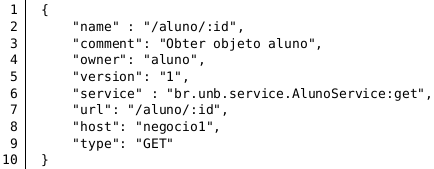
\includegraphics[scale=0.6]{figuras/catalogo.png}
\caption{Exemplo de catálogo de serviço para descrever o recurso aluno}
\label{fig:catalogo}
\end{figure}

O catálogo de serviço está sendo concebido para ser administrado a partir 
de um arquivo em formato JSON. Este arquivo deverá conter a descrição dos 
metadados que descrevem os serviços oferecidos pelo barramento. 
As informações contidas nesse catálogo seguem o modelo descrito 
por \cite{OASISRefArch:2012}. Entre as informações disponíveis estão 
o nome e a descrição do serviço, o responsável pelo serviço, a URL, 
os parâmetros do serviço, se o serviço é assíncrono ou não, entre outros dados.

Alguns requisitos técnicos para a arquitetura foram estipulados, como descritos a seguir:

\begin{enumerate}[(RQ1)]

\item Prover uma interface REST para comunicação com os clientes, por meio de uma API REST, suportando o subconjunto de operações HTTP \textit{GET, POST, PUT e DELETE}. 
O objetivo \'{e} fornecer uma tecnologia agnóstica sobre a linguagem de programa\c c\~{a}o
para troca de mensagens. Cada requisição deverá conter toda informação do 
pedido e nenhum estado das comunicações entre as mensagens deverá ser mantido. 
Além disso, cada recurso será unicamente direcionado através da sua URI.

\item Escalabilidade e tolerância a falhas (Requisito não funcional). Deve suportar 
duas características de qualidade de serviço (QoS): a escalabilidade 
(suportar uma carga de trabalho maior quando necessário) e tolerância a falhas 
(recuperar-se de possíveis falhas no processamento das solicitações). Além disso, 
uma requisição a um serviço de longa duração não deve comprometer o processamento 
das demais solicitações e qualquer falha no atendimento deverá retornar ao cliente 
na forma de uma mensagem JSON descrevendo o motivo do erro.

\item Monitoramento e Gerenciamento do Barramento. O barramento deverá prover um portal de gerenciamento, onde será possível monitorar o consumo dos serviços e listar 
os serviços disponíveis no catálogo.

\end{enumerate}


\subsection{Implementação do Barramento}

As características do projeto inicial foram trabalhadas na disciplina de \textit{Construção de Software} (CS). No primeiro seminário da disciplina, apresentou-se o protótipo da arquitetura do módulo HTTP (para suportar a interface de comunicação REST). Entre os desafios, destacam-se o parser do cabeçalho e a leitura completa do \textit{payload} da requisição HTTP.

Com a implementação do módulo HTTP, o próximo 
passo foi desenvolver o módulo de roteamento das requisições. Como não existia ainda um catálogo de serviço implementado, as rotas dos serviços 
foram inseridas diretamente no código fonte. Dois módulos de serviços foram criados 
para testar o roteamento preliminar: o serviço que trata a URL ‘‘/‘‘ e responde com a 
mensagem \{‘‘\textit{message}‘‘: ‘‘\textit{It works}‘‘\} e o serviço que trata 
a URL ‘‘/\textit{hello}\_\textit{world}‘‘ e retorna a 
mensagem \{‘‘\textit{message}‘‘: ‘‘Ola mundo‘‘\}.

Posteriormente, com a arquitetura básica pronta, o código foi refatorado com os princípios de design da \textit{Open Telecom Plataform} (OTP), 
o \textit{framework} da linguagem Erlang para construção de aplicações escaláveis e tolerante a falhas. Foram implementados o catálogo de serviços (a partir da leitura de um arquivo JSON), desenvolvido o módulo \textit{dispatcher} para localizar os serviços nesse catálogo (a partir da URL e do método HTTP da requisição) e redirecionar para o serviço correspondente. Também foi adicionado suporte para a transformação 
dos dados de/para JSON (de forma transparente dos processos de serviços) e 
implementado o tratamento de erros HTTP para os códigos de retorno mais comuns.

O próximo passo no desenvolvimento foi adicionar os recursos de supervisão da OTP 
(processos que supervisionam outros processos filhos) para gerar a árvore de supervisão 
e permitir ao barramento recuperar-se de possíveis falhas.

Para garantir a qualidade desejada, 62 testes automatizados foram gerados com a biblioteca Eunit (módulo para testes unitários do Erlang) para testar o funcionamento dos módulos implementados e simular requisições HTTP/REST (como um cliente faria) ao barramento de modo a analisar o comportamento do barramento durante sua execução.

As próximas versões do barramento vão focar na parte da integração dos processos em Java, utilizando a biblioteca \textit{jInterface} do Erlang. O desenvolvimento desta etapa será realizado em conjunto com a próxima etapa do trabalho, ou seja, durante o estudo de caso que será apresentado na próxima seção.


\section{Avaliação}\label{estudo-empirico}

Para que seja possível avaliar a abordagem proposta, surge a necessidade de aplicação em um ambiente real, de modo a investigar como a arquitetura comporta-se, quais os desafios técnicos e gerenciais, as dificuldades e os benefícios que podem ser obtidos com o seu uso.

Os estudos de caso tem sido utilizados normalmente para estes fins, de acordo com \cite{runeson2012case}, uma vez que, dão a oportunidade para que um aspecto de um problema seja estudado em profundidade, dentro de um período de tempo limitado (4 meses neste estudo). Além disso, parece ser apropriado como método de investigação, já que existem alguns fatores que devem ser observados quanto ao uso de uma abordagem orientada a serviço.

De forma resumida, o estudo visa modernizar o Sistema de Assistência Estudantil  (SAE) da UnB. Este sistema divide-se em dois módulos (1 módulo em VB e outro em C\#), ambos com duplicidades de implementação de regras de negócio e que o CPD tem interesse em modernizar. O trabalho que será realizado, envolve fazer uma análise estática dos códigos fontes para compreender o sistema, extrair a lógica negocial para uma camada de negócio que será criada em Java, desenvolver a fachada de serviços e registrar no catálogo de serviço. Por fim, a camada \textit{front-end} será modificada (ou reescrita a critério dos participantes do estudo de caso) para consumirem os serviços disponíveis no catálogo de serviços através do barramento.

A avaliação será aplicada com 9 pessoas: 7 analistas do CPD e 2 alunos da Universidade. Todos os participantes estão cursando a disciplina \textit{Modernização de Software} do Mestrado Acadêmico em Informática da UnB, que vai apoiar este estudo. Os papéis serão delineados no decorrer da avaliação, conforme o perfil de cada integrante. Será avaliado a produtividade alcançada a partir de um questionário aplicado com os integrantes do estudo e estimado o tamanho do código fonte através da métrica LOC (\textit{Line of Code)} para fazer comparações com o sistema legado e verificar algumas questões modularidade (coesão, acoplamento) e possível redução de duplicidade de implementação das regras de negócio.




\section{Considerações Finais}\label{sec:final-remarks}

A modernização dos sistemas legados tem ganhado muita atenção nos últimos anos, levando
a um número de contribuições de pesquisa que apresentam novos métodos, técnicas e ferramentas. No entanto, a falta de uma consolidação adequada destes resultados dificulta tanto pesquisadores quanto profissionais de realizarem as suas atividades, bem como de descreverem as suas descobertas e experiências usando um conhecimento comum. Neste artigo foi apresentado os primeiro resultado de um estudo de mapeamento (MS) submetido ao ACM SAC 2016, a qual, consolidou as principais contribuições para o campo; e detalhou-se as experiências de modernização de software na Universidade de Bras\'{i}lia, de acordo com alguns resultados dos MS e do estudo de caso que está sendo conduzido para fazer a modernização de um sistema legado em uso na Instituição através de uma abordagem orientada a serviço. 



\bibliographystyle{plain}
\bibliography{bibliografia}

% that's all folks
\end{document}

